% !TeX program = xelatex 

\PassOptionsToPackage{prologue, dvipsnames}{xcolor}
\documentclass[AutoFakeBold,AutoFakeSlant]{article}
\usepackage{listings}

% 支持中文的设置
\usepackage{xeCJK}
\usepackage{fontspec}
\setCJKmainfont[ItalicFont=思源宋体,BoldFont=SourceHanSerifSC-Bold]{Source Han Serif SC}
\newcommand{\KaiTi}{\CJKfontspec{楷体}}%用命令\fzkaiti调用方正楷体简体

% other packages
\usepackage{subfigure}
\usepackage{latexsym,amsmath,xcolor,multicol,booktabs,calligra}
\usepackage{graphicx,pstricks,listings,stackengine}

\usepackage{geometry}
\geometry{left=2cm,right=2cm,top=2cm,bottom=2cm}

\lstnewenvironment{cppcode}[1][]%
{
	\lstset{
		tabsize=4,
		language={C++},
		escapeinside=``,
		breaklines=true,
		breakatwhitespace=true, % 在空格处断行
		basicstyle=\ttfamily,
		keywordstyle=\color{blue}\ttfamily,
		stringstyle=\color{red}\ttfamily,
		commentstyle=\color{green}\ttfamily,
		morecomment=[l][\color{magenta}]{\#},
		literate={\ \ }{{\ \ \ \ }}4,
		#1
	}
}%
{}

\begin{document}
	
	\begin{center}
		\Huge 
		CEF Cookie 请求问题
	\end{center}
	
	\leftline
	\bigskip
	\begin{flushleft}
		\begin{huge}
			一、 情景描述
		\end{huge}
		
		\large 
		\linespread{1.2} \selectfont
		基于cefsimple工程中的SimpleApp::OnContextInitialized中的
		url="http://www.google.com"
		改成
		url = "http://10.10.10.239:2342";
		
		\bigskip
		
		通过抓包工具查看,设置过滤条件:\\	
		ip.addr == 10.10.10.239 \&\& tcp.port == 2342
	\end{flushleft}
	
	
	
	\begin{flushleft}
		\begin{figure*}[htbp]
			\centering
			\subfigure[在没有设置cookie之前]{
				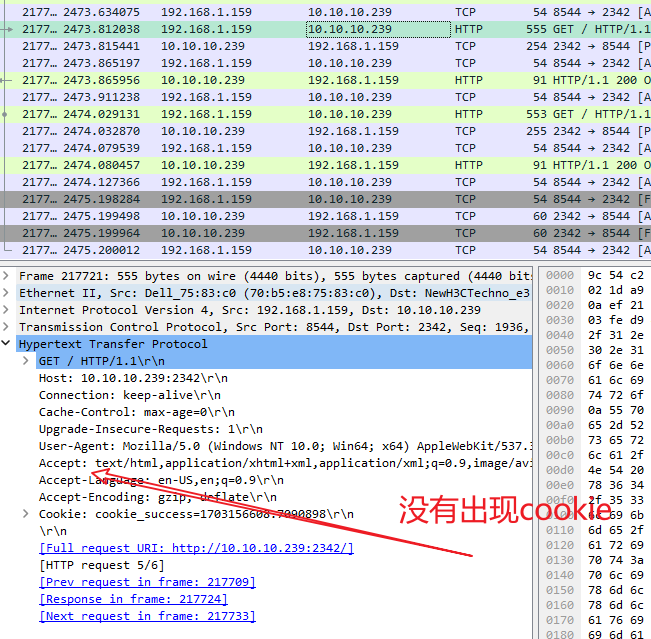
\includegraphics[width=0.7\linewidth]{1}
			} 
			
			\vspace{1cm}
			
			\subfigure[响应页面结果]{
			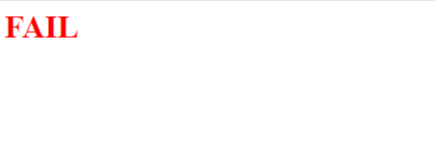
\includegraphics[width=0.3\linewidth]{NG}
			} 
		\end{figure*}
	\end{flushleft}
	
	\newpage
	
	
	\begin{flushleft}
		\begin{huge}
			二、 问题描述
		\end{huge}
		
		\large 
		\linespread{1.2} \selectfont
		如何修改OnContextInitialized中的代码,或者其他位置的代码,使其出现:
	\end{flushleft}
	\begin{flushleft}
		\begin{figure*}[htbp]
			\centering
			\subfigure[在没有设置cookie之前]{
				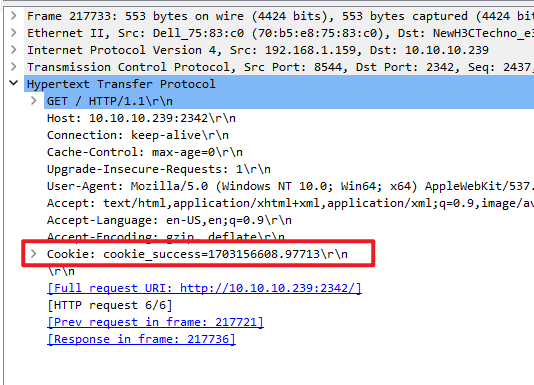
\includegraphics[width=0.7\linewidth]{2}
			} 
			
			\vspace{1cm}
			
			\subfigure[响应页面结果]{
				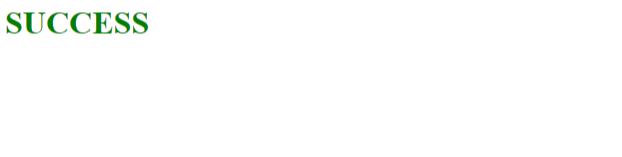
\includegraphics[width=0.3\linewidth]{OK}
			} 
		\end{figure*}
	\end{flushleft}
	
	\clearpage
	
	\begin{flushleft}
		\begin{huge}
			三、 目前的研究
		\end{huge}
		
		\bigskip
		
		\large 
		\linespread{1.2} \selectfont
		\textbf{实现方式1:}
		\begin{cppcode}
	// 创建 CefRequest 对象
	CefRefPtr<CefRequest> request = CefRequest::Create();
	request->SetURL("http://10.10.10.239:2342/");
	
	CefRequest::HeaderMap headerMap;
	headerMap.insert({"Cookie", name + "=" + value});
	request->SetHeaderMap(headerMap);
	
	// 创建 CefURLRequest 实例并发送请求
	CefRefPtr<CefURLRequest> urlRequest =
	CefURLRequest::Create(request, new MyRequestClient(), nullptr);
		\end{cppcode}
		这种方式虽然能将cookie正确和Get请求发送,但是奇怪的是响应页面并没有渲染窗口上???
		
		\vspace{2cm}
		
		\large 
		\linespread{1.2} \selectfont
		\textbf{实现方式2:}
		\begin{cppcode}
	bool SimpleHandler::OnBeforeBrowse(
	  CefRefPtr<CefBrowser> browser,
	  CefRefPtr<CefFrame> frame,
	  CefRefPtr<CefRequest> request,
	  bool user_gesture,
	  bool is_redirect) {
		// Check if the request is for a specific domain
		CefString url = request->GetURL();
		request->SetURL("https://www.baidu.com/");
		url = request->GetURL();
		
		// Continue with the request
		return false;
	}
		\end{cppcode}
		这种方式可以在发送数据到服务器之前断下,但是由于request对象是只读的,导致设置新的URL等写操作无效,原本想在发送之前在这里加入cookie,但是现在因为只读的原因无法达成,如果这里能修改requst的内容,效果是最好的.
	\end{flushleft}
	
\end{document}
